% Options for packages loaded elsewhere
\PassOptionsToPackage{unicode}{hyperref}
\PassOptionsToPackage{hyphens}{url}
%
\documentclass[
]{book}

\usepackage{amsmath,amssymb}
\usepackage{lmodern}
\usepackage{iftex}
\ifPDFTeX
  \usepackage[T1]{fontenc}
  \usepackage[utf8]{inputenc}
  \usepackage{textcomp} % provide euro and other symbols
\else % if luatex or xetex
  \usepackage{unicode-math}
  \defaultfontfeatures{Scale=MatchLowercase}
  \defaultfontfeatures[\rmfamily]{Ligatures=TeX,Scale=1}
\fi
% Use upquote if available, for straight quotes in verbatim environments
\IfFileExists{upquote.sty}{\usepackage{upquote}}{}
\IfFileExists{microtype.sty}{% use microtype if available
  \usepackage[]{microtype}
  \UseMicrotypeSet[protrusion]{basicmath} % disable protrusion for tt fonts
}{}
\makeatletter
\@ifundefined{KOMAClassName}{% if non-KOMA class
  \IfFileExists{parskip.sty}{%
    \usepackage{parskip}
  }{% else
    \setlength{\parindent}{0pt}
    \setlength{\parskip}{6pt plus 2pt minus 1pt}}
}{% if KOMA class
  \KOMAoptions{parskip=half}}
\makeatother
\usepackage{xcolor}
\usepackage[margin=1.5in]{geometry}
\usepackage{color}
\usepackage{fancyvrb}
\newcommand{\VerbBar}{|}
\newcommand{\VERB}{\Verb[commandchars=\\\{\}]}
\DefineVerbatimEnvironment{Highlighting}{Verbatim}{commandchars=\\\{\}}
% Add ',fontsize=\small' for more characters per line
\usepackage{framed}
\definecolor{shadecolor}{RGB}{248,248,248}
\newenvironment{Shaded}{\begin{snugshade}}{\end{snugshade}}
\newcommand{\AlertTok}[1]{\textcolor[rgb]{0.94,0.16,0.16}{#1}}
\newcommand{\AnnotationTok}[1]{\textcolor[rgb]{0.56,0.35,0.01}{\textbf{\textit{#1}}}}
\newcommand{\AttributeTok}[1]{\textcolor[rgb]{0.77,0.63,0.00}{#1}}
\newcommand{\BaseNTok}[1]{\textcolor[rgb]{0.00,0.00,0.81}{#1}}
\newcommand{\BuiltInTok}[1]{#1}
\newcommand{\CharTok}[1]{\textcolor[rgb]{0.31,0.60,0.02}{#1}}
\newcommand{\CommentTok}[1]{\textcolor[rgb]{0.56,0.35,0.01}{\textit{#1}}}
\newcommand{\CommentVarTok}[1]{\textcolor[rgb]{0.56,0.35,0.01}{\textbf{\textit{#1}}}}
\newcommand{\ConstantTok}[1]{\textcolor[rgb]{0.00,0.00,0.00}{#1}}
\newcommand{\ControlFlowTok}[1]{\textcolor[rgb]{0.13,0.29,0.53}{\textbf{#1}}}
\newcommand{\DataTypeTok}[1]{\textcolor[rgb]{0.13,0.29,0.53}{#1}}
\newcommand{\DecValTok}[1]{\textcolor[rgb]{0.00,0.00,0.81}{#1}}
\newcommand{\DocumentationTok}[1]{\textcolor[rgb]{0.56,0.35,0.01}{\textbf{\textit{#1}}}}
\newcommand{\ErrorTok}[1]{\textcolor[rgb]{0.64,0.00,0.00}{\textbf{#1}}}
\newcommand{\ExtensionTok}[1]{#1}
\newcommand{\FloatTok}[1]{\textcolor[rgb]{0.00,0.00,0.81}{#1}}
\newcommand{\FunctionTok}[1]{\textcolor[rgb]{0.00,0.00,0.00}{#1}}
\newcommand{\ImportTok}[1]{#1}
\newcommand{\InformationTok}[1]{\textcolor[rgb]{0.56,0.35,0.01}{\textbf{\textit{#1}}}}
\newcommand{\KeywordTok}[1]{\textcolor[rgb]{0.13,0.29,0.53}{\textbf{#1}}}
\newcommand{\NormalTok}[1]{#1}
\newcommand{\OperatorTok}[1]{\textcolor[rgb]{0.81,0.36,0.00}{\textbf{#1}}}
\newcommand{\OtherTok}[1]{\textcolor[rgb]{0.56,0.35,0.01}{#1}}
\newcommand{\PreprocessorTok}[1]{\textcolor[rgb]{0.56,0.35,0.01}{\textit{#1}}}
\newcommand{\RegionMarkerTok}[1]{#1}
\newcommand{\SpecialCharTok}[1]{\textcolor[rgb]{0.00,0.00,0.00}{#1}}
\newcommand{\SpecialStringTok}[1]{\textcolor[rgb]{0.31,0.60,0.02}{#1}}
\newcommand{\StringTok}[1]{\textcolor[rgb]{0.31,0.60,0.02}{#1}}
\newcommand{\VariableTok}[1]{\textcolor[rgb]{0.00,0.00,0.00}{#1}}
\newcommand{\VerbatimStringTok}[1]{\textcolor[rgb]{0.31,0.60,0.02}{#1}}
\newcommand{\WarningTok}[1]{\textcolor[rgb]{0.56,0.35,0.01}{\textbf{\textit{#1}}}}
\usepackage{longtable,booktabs,array}
\usepackage{calc} % for calculating minipage widths
% Correct order of tables after \paragraph or \subparagraph
\usepackage{etoolbox}
\makeatletter
\patchcmd\longtable{\par}{\if@noskipsec\mbox{}\fi\par}{}{}
\makeatother
% Allow footnotes in longtable head/foot
\IfFileExists{footnotehyper.sty}{\usepackage{footnotehyper}}{\usepackage{footnote}}
\makesavenoteenv{longtable}
\usepackage{graphicx}
\makeatletter
\def\maxwidth{\ifdim\Gin@nat@width>\linewidth\linewidth\else\Gin@nat@width\fi}
\def\maxheight{\ifdim\Gin@nat@height>\textheight\textheight\else\Gin@nat@height\fi}
\makeatother
% Scale images if necessary, so that they will not overflow the page
% margins by default, and it is still possible to overwrite the defaults
% using explicit options in \includegraphics[width, height, ...]{}
\setkeys{Gin}{width=\maxwidth,height=\maxheight,keepaspectratio}
% Set default figure placement to htbp
\makeatletter
\def\fps@figure{htbp}
\makeatother
\setlength{\emergencystretch}{3em} % prevent overfull lines
\providecommand{\tightlist}{%
  \setlength{\itemsep}{0pt}\setlength{\parskip}{0pt}}
\setcounter{secnumdepth}{5}
\usepackage{booktabs}

\usepackage{epsfig}
\usepackage{epstopdf}
\usepackage{rotate}
\usepackage{graphicx}
\usepackage{hyperref}
\usepackage{alphalph}
\usepackage{caption}
\usepackage[hang,flushmargin]{footmisc}
\usepackage{framed}
\usepackage{xcolor}
\usepackage{verbatim} 

\usepackage{bm}
\setcounter{MaxMatrixCols}{20}
\newcommand{\Var}{\mathrm{Var}}
\newcommand{\SD}{\mathrm{SD}}
\newcommand{\Cov}{\mathrm{Cov}}
\newcommand{\fx}{f({\bf x})}
\newcommand\R{{\textsf R~}}
\newcommand\Rst{\textsf{RStudio}}

% spacing between environments
\usepackage{amsthm}
\makeatletter
\def\thm@space@setup{%
  \thm@preskip=15pt plus 2pt minus 4pt
  \thm@postskip=\thm@preskip
}
\makeatother

% link colors in pdf?
\usepackage{xcolor}  
\definecolor{crimson}{RGB}{204,0,0}
\hypersetup{
  colorlinks = true,
  urlcolor = crimson,
  linkbordercolor = {white},
  linkcolor = crimson
}


% Title format
\usepackage{titling}
\pretitle{\Huge\sffamily}
\posttitle{\par\vskip 1em}
\predate{\LARGE\sffamily}
\postdate{\par}

\urlstyle{tt}
\ifLuaTeX
  \usepackage{selnolig}  % disable illegal ligatures
\fi
\usepackage[]{natbib}
\bibliographystyle{apalike}
\IfFileExists{bookmark.sty}{\usepackage{bookmark}}{\usepackage{hyperref}}
\IfFileExists{xurl.sty}{\usepackage{xurl}}{} % add URL line breaks if available
\urlstyle{same} % disable monospaced font for URLs
\hypersetup{
  pdftitle={Math Prefresher for Political Scientists},
  hidelinks,
  pdfcreator={LaTeX via pandoc}}

\title{Math Prefresher for Political Scientists}
\author{}
\date{\vspace{-2.5em}August 2023}

\usepackage{amsthm}
\newtheorem{theorem}{Theorem}[chapter]
\newtheorem{lemma}{Lemma}[chapter]
\newtheorem{corollary}{Corollary}[chapter]
\newtheorem{proposition}{Proposition}[chapter]
\newtheorem{conjecture}{Conjecture}[chapter]
\theoremstyle{definition}
\newtheorem{definition}{Definition}[chapter]
\theoremstyle{definition}
\newtheorem{example}{Example}[chapter]
\theoremstyle{definition}
\newtheorem{exercise}{Pencil Problem}[chapter]
\theoremstyle{definition}
\newtheorem{hypothesis}{Hypothesis}[chapter]
\theoremstyle{remark}
\newtheorem*{remark}{Remark}
\newtheorem*{solution}{Solution}

\DeclareUnicodeCharacter{2212}{-}


\begin{document}

\setcounter{chapter}{3}
\setcounter{section}{6}

\hypertarget{the-indefinite-integration}{%
\section{The Indefinite Integration}\label{the-indefinite-integration}}

So far, we've been interested in finding the derivative \(f=F'\) of a function \(F\). However, sometimes we're interested in exactly the reverse: finding the function \(F\) for which \(f\) is its derivative. We refer to \(F\) as the antiderivative of \(f\).

\begin{definition}[Antiderivative]
\protect\hypertarget{def:unnamed-chunk-20}{}\label{def:unnamed-chunk-20}The antiverivative of a function \(f(x)\) is a differentiable function \(F\) whose derivative is \(f\).

\[F^\prime = f.\]
\end{definition}

Another way to describe is through the inverse formula. Let \(DF\) be the derivative of \(F\). And let \(DF(x)\) be the derivative of \(F\) evaluated at \(x\). Then the antiderivative is denoted by \(D^{-1}\) (i.e., the inverse derivative). If \(DF=f\), then \(F=D^{-1}f\).

This definition bolsters the main takeaway about integrals and derivatives: They are inverses of each other.

\begin{exercise}[Antiderivative]
\protect\hypertarget{exr:unnamed-chunk-21}{}\label{exr:unnamed-chunk-21}

Find the antiderivative of the following:

\begin{enumerate}
\def\labelenumi{\arabic{enumi}.}
\tightlist
\item
  \(f(x) = \frac{1}{x^2}\)
\item
  \(f(x) = 3e^{3x}\)
\end{enumerate}

\end{exercise}

We know from derivatives how to manipulate \(F\) to get \(f\). But how do you express the procedure to manipulate \(f\) to get \(F\)? For that, we need a new symbol, which we will call indefinite integration.

\begin{definition}[Indefinite Integral]
\protect\hypertarget{def:unnamed-chunk-22}{}\label{def:unnamed-chunk-22}The indefinite integral of \(f(x)\) is written

\[\int f(x) dx \]

and is equal to the antiderivative of \(f\).
\end{definition}

\begin{example}
\protect\hypertarget{exm:unnamed-chunk-23}{}\label{exm:unnamed-chunk-23}Draw the function \(f(x)\) and its indefinite integral, \(\int\limits f(x) dx\)

\[f(x) = (x^2-4)\]
\end{example}

\begin{solution}
The Indefinite Integral of the function \(f(x) = (x^2-4)\) can, for example, be \(F(x) = \frac{1}{3}x^3 - 4x.\) But it can also be \(F(x) = \frac{1}{3}x^3 - 4x + 1\), because the constant 1 disappears when taking the derivative.
\end{solution}

Some of these functions are plotted in the bottom panel of Figure \ref{fig:integralc} as dotted lines.

\begin{figure}
\centering
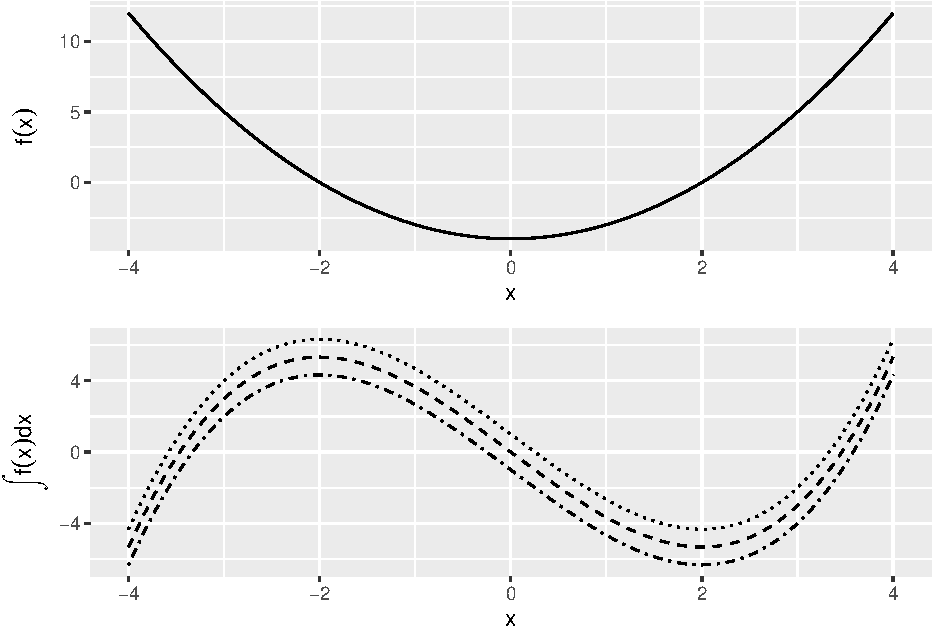
\includegraphics{figure-latex/integralc-1.pdf}
\caption{\label{fig:integralc}The Many Indefinite Integrals of a Function}
\end{figure}

Notice from these examples that while there is only a single derivative for any function, there are multiple antiderivatives: one for any arbitrary constant \(c\). \(c\) just shifts the curve up or down on the \(y\)-axis. If more information is present about the antiderivative --- e.g., that it passes through a particular point --- then we can solve for a specific value of \(c\).

\hypertarget{common-rules-of-integration}{%
\subsection*{Common Rules of Integration}\label{common-rules-of-integration}}
\addcontentsline{toc}{subsection}{Common Rules of Integration}

Some common rules of integrals follow by virtue of being the inverse of a derivative.

\begin{enumerate}
\def\labelenumi{\arabic{enumi}.}
\tightlist
\item
  Constants are allowed to slip out: \(\int a f(x)dx = a\int f(x)dx\)
\item
  Integration of the sum is sum of integrations: \(\int [f(x)+g(x)]dx=\int f(x)dx + \int g(x)dx\)
\item
  Reverse Power-rule: \(\int x^n dx = \frac{1}{n+1} x^{n+1} + c\)
\item
  Exponents are still exponents: \(\int e^x dx = e^x +c\)
\item
  Recall the derivative of \(\log(x)\) is one over \(x\), and so: \(\int \frac{1}{x} dx = \log x + c\)
\item
  Reverse chain-rule: \(\int e^{f(x)}f^\prime(x)dx = e^{f(x)}+c\)
\item
  More generally: \(\int [f(x)]^n f'(x)dx = \frac{1}{n+1}[f(x)]^{n+1}+c\)
\item
  Remember the derivative of a log of a function: \(\int \frac{f^\prime(x)}{f(x)}dx=\log f(x) + c\)
\end{enumerate}

\begin{example}[Common Integration]
\protect\hypertarget{exm:unnamed-chunk-25}{}\label{exm:unnamed-chunk-25}

Simplify the following indefinite integrals:

\begin{itemize}
\tightlist
\item
  \(\int 3x^2 dx\)
\item
  \(\int (2x+1)dx\)
\item
  \(\int e^x e^{e^x} dx\)
\end{itemize}

\end{example}

\hypertarget{the-definite-integral-the-area-under-the-curve}{%
\section{The Definite Integral: The Area under the Curve}\label{the-definite-integral-the-area-under-the-curve}}

If there is a indefinite integral, there \emph{must} be a definite integral. Indeed there is, but the notion of definite integrals comes from a different objective: finding the are a under a function. We will find, perhaps remarkably, that the formula we find to get the sum turns out to be expressible by the anti-derivative.

Suppose we want to determine the area \(A(R)\) of a region \(R\) defined by a curve \(f(x)\) and some interval \(a\le x \le b\).

\begin{figure}
\centering
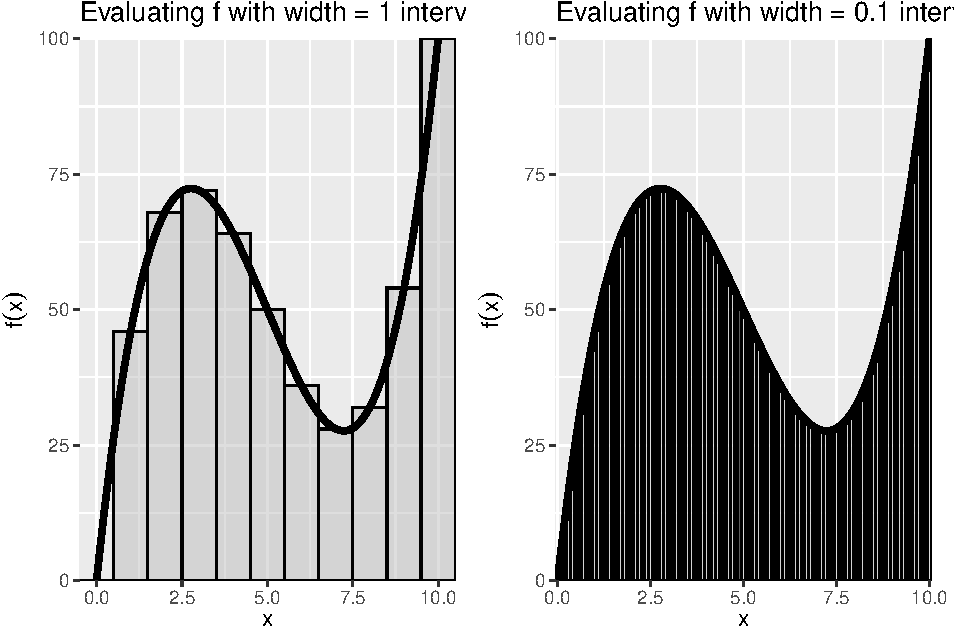
\includegraphics{figure-latex/defintfig-1.pdf}
\caption{\label{fig:defintfig}The Riemann Integral as a Sum of Evaluations}
\end{figure}

One way to calculate the area would be to divide the interval \(a\le x\le b\) into \(n\) subintervals of length \(\Delta x\) and then approximate the region with a series of rectangles, where the base of each rectangle is \(\Delta x\) and the height is \(f(x)\) at the midpoint of that interval. \(A(R)\) would then be approximated by the area of the union of the rectangles, which is given by \[S(f,\Delta x)=\sum\limits_{i=1}^n f(x_i)\Delta x\] and is called a \textbf{Riemann sum}.

As we decrease the size of the subintervals \(\Delta x\), making the rectangles ``thinner,'' we would expect our approximation of the area of the region to become closer to the true area. This allows us to express the area as a limit of a series:
\[A(R)=\lim\limits_{\Delta x\to 0}\sum\limits_{i=1}^n f(x_i)\Delta x\]

Figure \ref{fig:defintfig} shows that illustration. The curve depicted is \(f(x) = -15(x - 5) + (x - 5)^3 + 50.\) We want approximate the area under the curve between the \(x\) values of 0 and 10. We can do this in blocks of arbitrary width, where the sum of rectangles (the area of which is width times \(f(x)\) evaluated at the midpoint of the bar) shows the Riemann Sum. As the width of the bars \(\Delta x\) becomes smaller, the better the estimate of \(A(R)\).

This is how we define the ``Definite'' Integral:

\begin{definition}[The Definite Integral (Riemann)]
\protect\hypertarget{def:unnamed-chunk-26}{}\label{def:unnamed-chunk-26}If for a given function \(f\) the Riemann sum approaches a limit as \(\Delta x \to 0\), then that limit is called the Riemann integral of \(f\) from \(a\) to \(b\). We express this with the \(\int\), symbol, and write \[\int\limits_a^b f(x) dx= \lim\limits_{\Delta x\to 0} \sum\limits_{i=1}^n f(x_i)\Delta x\]

The most straightforward of a definite integral is the definite integral. That is, we read
\[\int\limits_a^b f(x) dx\] as the definite integral of \(f\) from \(a\) to \(b\) and we defined as the area under the ``curve'' \(f(x)\) from point \(x=a\) to \(x=b\).
\end{definition}

The fundamental theorem of calculus shows us that this sum is, in fact, the antiderivative.

\begin{theorem}[First Fundamental Theorem of Calculus]
\protect\hypertarget{thm:unnamed-chunk-27}{}\label{thm:unnamed-chunk-27}Let the function \(f\) be bounded on \([a,b]\) and continuous on \((a,b)\). Then, suggestively, use the symbol \(F(x)\) to denote the definite integral from \(a\) to \(x\):
\[F(x)=\int\limits_a^x f(t)dt, \quad a\le x\le b\]

Then \(F(x)\) has a derivative at each point in \((a,b)\) and \[F^\prime(x)=f(x), \quad a<x<b\]
That is, the definite integral function of \(f\) \emph{is} the one of the antiderivatives of some \(f\).
\end{theorem}

This is again a long way of saying that that differentiation is the inverse of integration. But now, we've covered definite integrals.

The second theorem gives us a simple way of computing a definite integral as a function of indefinite integrals.

\begin{theorem}[Second Fundamental Theorem of Calculus]
\protect\hypertarget{thm:unnamed-chunk-28}{}\label{thm:unnamed-chunk-28}Let the function \(f\) be bounded on \([a,b]\) and continuous on \((a,b)\). Let \(F\) be any function that is continuous on \([a,b]\) such that \(F^\prime(x)=f(x)\) on \((a,b)\). Then \[\int\limits_a^bf(x)dx = F(b)-F(a)\]
\end{theorem}

So the procedure to calculate a simple definite integral \(\int\limits_a^b f(x)dx\) is then

\begin{enumerate}
\def\labelenumi{\arabic{enumi}.}
\tightlist
\item
  Find the indefinite integral \(F(x)\).
\item
  Evaluate \(F(b)-F(a)\).
\end{enumerate}

\begin{example}[Definite Integral of a monomial]
\protect\hypertarget{exm:defintmon}{}\label{exm:defintmon}Solve \(\int\limits_1^3 3x^2 dx.\)

Let \(f(x) = 3x^2\).
\end{example}

\begin{exercise}
\protect\hypertarget{exr:unnamed-chunk-29}{}\label{exr:unnamed-chunk-29}What is the value of \(\int\limits_{-2}^2 e^x e^{e^x} dx\)?
\end{exercise}

\hypertarget{common-rules-for-definite-integrals}{%
\subsection*{Common Rules for Definite Integrals}\label{common-rules-for-definite-integrals}}
\addcontentsline{toc}{subsection}{Common Rules for Definite Integrals}

The area-interpretation of the definite integral provides some rules for simplification.

\begin{enumerate}
\def\labelenumi{\arabic{enumi}.}
\tightlist
\item
  There is no area below a point: \[\int\limits_a^a f(x)dx=0\]
\item
  Reversing the limits changes the sign of the integral: \[\int\limits_a^b f(x)dx=-\int\limits_b^a f(x)dx\]
\item
  Sums can be separated into their own integrals: \[\int\limits_a^b [\alpha f(x)+\beta g(x)]dx = \alpha \int\limits_a^b f(x)dx + \beta \int\limits_a^b g(x)dx\]
\item
  Areas can be combined as long as limits are linked: \[\int\limits_a^b f(x) dx +\int\limits_b^c f(x)dx = \int\limits_a^c f(x)dx\]
\end{enumerate}

\begin{exercise}[Definite integral shortcuts]
\protect\hypertarget{exr:unnamed-chunk-30}{}\label{exr:unnamed-chunk-30}

Simplify the following definite intergrals.

\begin{enumerate}
\def\labelenumi{\arabic{enumi}.}
\tightlist
\item
  \(\int\limits_1^1 3x^2 dx =\)
\item
  \(\int\limits_0^4 (2x+1)dx=\)
\item
  \(\int\limits_{-2}^0 e^x e^{e^x} dx + \int\limits_0^2 e^x e^{e^x} dx =\)
\end{enumerate}

\end{exercise}

\hypertarget{integration-by-substitution}{%
\section{Integration by Substitution}\label{integration-by-substitution}}

From the second fundamental theorem of calculus, we now that a quick way to get a definite integral is to first find the indefinite integral, and then just plug in the bounds.

Sometimes the integrand (the thing that we are trying to take an integral of) doesn't appear integrable using common rules and antiderivatives. A method one might try is \textbf{integration by substitution}, which is related to the Chain Rule.

Suppose we want to find the indefinite integral \[\int g(x)dx\] but \(g(x)\) is complex and none of the formulas we have seen so far seem to apply immediately. The trick is to come up with a \emph{new} function \(u(x)\) such that \[g(x)=f[u(x)]u'(x).\]

Why does an introduction of yet another function end of simplifying things? Let's refer to the antiderivative of \(f\) as \(F\). Then the chain rule tells us that \[\frac{d}{dx} F[u(x)]=f[u(x)]u'(x)\]. So, \(F[u(x)]\) is the antiderivative of \(g\). We can then write \[\int g(x) dx= \int f[u(x)]u'(x)dx = \int \frac{d}{dx} F[u(x)]dx = F[u(x)]+c\]

To summarize, the procedure to determine the indefinite integral \(\int g(x)dx\) by the method of substitution:

\begin{enumerate}
\def\labelenumi{\arabic{enumi}.}
\tightlist
\item
  Identify some part of \(g(x)\) that might be simplified by substituting in a single variable \(u\) (which will then be a function of \(x\)).
\item
  Determine if \(g(x)dx\) can be reformulated in terms of \(u\) and \(du\).
\item
  Solve the indefinite integral.
\item
  Substitute back in for \(x\)
\end{enumerate}

Substitution can also be used to calculate a definite integral. Using the same procedure as above, \[\int\limits_a^b g(x)dx=\int\limits_c^d f(u)du = F(d)-F(c)\]
where \(c=u(a)\) and \(d=u(b)\).

\begin{example}[Integration by Substitution I]
\protect\hypertarget{exm:intsub1}{}\label{exm:intsub1}Solve the indefinite integral \[\int x^2 \sqrt{x+1}dx.\]
\end{example}

For the above problem, we could have also used the substitution \(u=\sqrt{x+1}\). Then \(x=u^2-1\) and \(dx=2u du\). Substituting these in, we get \[\int x^2\sqrt{x+1}dx=\int (u^2-1)^2 u 2u du\] which when expanded is again a polynomial and gives the same result as above.

Another case in which integration by substitution is is useful is with a fraction.

\begin{example}[Integration by Substitutiton II]
\protect\hypertarget{exm:intsub2}{}\label{exm:intsub2}Simplify \[\int\limits_0^1 \frac{5e^{2x}}{(1+e^{2x})^{1/3}}dx.\]
\end{example}

\hypertarget{integration-by-parts}{%
\section{Integration by Parts}\label{integration-by-parts}}

Another useful integration technique is \textbf{integration by parts}, which is related to the Product Rule of differentiation. The product rule states that \[\frac{d}{dx}(uv)=u\frac{dv}{dx}+v\frac{du}{dx}\] Integrating this and rearranging, we get \[\int u\frac{dv}{dx}dx= u v - \int v \frac{du}{dx}dx\] or \[\int u(x) v'(x)dx=u(x)v(x) - \int v(x)u'(x)dx\]

More easily remembered with the mnemonic ``Ultraviolet Voodoo'': \[\int u dv = u v - \int v du\] where \(du=u'(x)dx\) and \(dv=v'(x)dx\).

For definite integrals, this is simply
\[\int\limits_a^b u\frac{dv}{dx}dx = \left. u v \right|_a^b - \int\limits_a^b v \frac{du}{dx}dx\]

Our goal here is to find expressions for \(u\) and \(dv\) that, when substituted into the above equation, yield an expression that's more easily evaluated.

\begin{example}[Integration by Parts]
\protect\hypertarget{exm:unnamed-chunk-31}{}\label{exm:unnamed-chunk-31}Simplify the following integrals. These seemingly obscure forms of integrals come up often when integrating distributions.

\[\int x e^{ax} dx\]
\end{example}

\begin{solution}
Let \(u=x\) and \(\frac{dv}{dx} = e^{ax}\). Then \(du=dx\) and \(v=(1/a)e^{ax}\). Substituting this into the integration by parts formula, we obtain\\
\begin{eqnarray}
\int x e^{ax} dx &=& u v - \int v du\nonumber\\
                &=&x\left( \frac{1}{a}e^{ax}\right) -\int\frac{1}{a}e^{ax}dx\nonumber\\
                &=&\frac{1}{a}xe^{ax}-\frac{1}{a^2}e^{ax}+c\nonumber
\end{eqnarray}
\end{solution}

\begin{exercise}[Integration by Parts II]
\protect\hypertarget{exr:intparts-adv}{}\label{exr:intparts-adv}

\begin{enumerate}
\def\labelenumi{\arabic{enumi}.}
\item
  Integrate
  \[\int x^n e^{ax} dx\]
\item
  Integrate
  \[\int x^3 e^{-x^2} dx\]
\end{enumerate}

\end{exercise}

\hypertarget{optim}{%
\chapter{Optimization}\label{optim}}

To optimize, we use derivatives and calculus. Optimization is to find the maximum or minimum of a functon, and to find what value of an input gives that extremum. This has obvious uses in engineering. Many tools in the statistical toolkit use optimization. One of the most common ways of estimating a model is through ``Maximum Likelihood Estimation'', done via optimizing a function (the likelihood).

Optimization also comes up in Economics, Formal Theory, and Political Economy all the time. A go-to model of human behavior is that they optimize a certain utility function. Humans are not pure utility maximizers, of course, but nuanced models of optimization -- for example, adding constraints and adding uncertainty -- will prove to be quite useful.

\hypertarget{example-meltzer-richard}{%
\section*{Example: Meltzer-Richard}\label{example-meltzer-richard}}
\addcontentsline{toc}{section}{Example: Meltzer-Richard}

A standard backdrop in comparative political economy, the Meltzer-Richard (1981) model states that redistribution of wealth should be higher in societies where the median income is much smaller than the average income. More to the point, typically income distributions wher ethe median is very different from the average is one of high inequality. In other words, the Meltzer-Richard model says that highly unequal economies will have more re-distribution of wealth. Why is that the case? Here is a simplified example that is not the exact model by Meltzer and Richard\footnote{Allan H. Meltzer and Scott F. Richard. \href{https://www.jstor.org/stable/1830813}{``A Rational Theory of the Size of Government''}. \emph{Journal of Political Economy}
  89:5 (1981), p.~914-927}, but adapted from Persson and Tabellini\footnote{Adapted from Torsten Persson and Guido Tabellini, \emph{Political Economics: Explaining Economic Policy}. MIT Press.}

We will set the following things about our model human and model democracy.

\begin{itemize}
\tightlist
\item
  Individuals are indexed by \(i\), and the total population is normalized to unity (``1'') without loss of generality.
\item
  \(U(\cdot)\), u for ``utility'', is a function that is concave and increasing, and expresses the utility gained from public goods. This tells us that its first derivative is \emph{positive}, and its second derivative is \textbf{negative}.
\item
  \(y_i\) is the income of person \(i\)
\item
  \(W_i\), w for ``welfare'', is the welfare of person \(i\)
\item
  \(c_i\), c for ``consumption'', is the consumption utility of person \(i\)
\end{itemize}

Also, the government is democratically elected and sets the following redistribution output:

\begin{itemize}
\tightlist
\item
  \(\tau\), t for ``tax'', is a flat tax rate between 0 and 1 that is applied to everyone's income.
\item
  \(g\), ``g'' for ``goods'', is the amount of public goods that the government provides.
\end{itemize}

Suppose an individual's welfare is given by:
\[W_i = c_i + U(g)\]

The consumption good is the person's post-tax income.

\[c_i = (1 - \tau) y_i\]

Income varies by person (In the next section we will cover probability, by then we will know that we can express this by saying that \(y\) is a random variable with the cumulative distribution function \(F\), i.e.~\(y \sim F\).). Every distribution has a mean and an median.

\begin{itemize}
\tightlist
\item
  \(E(y)\) is the average income of the society.
\item
  \(\text{med}(y)\) is the \textbf{median income} of the society.
\end{itemize}

What will happen in this economy? What will the tax rate be set too? How much public goods will be provided?

We've skipped ahead of some formal theory results of demoracy, but hopefully these are conceptually intuitive. First, if a democracy is competitive, there is no slack in the government's goods, and all tax revenue becomes a public good. So we can go ahead and set the constraint:

\[g = \sum_{i} \tau y_i P(y_i) = \tau E(y)\]

We can do this trick because of the ``normalizes to unity'' setting, but this is a general property of the average.

Now given this constraint we can re-write an individual's welfare as

\begin{align*}
W_i &= \left(1 - \frac{g}{E(y)}\right)y_i + U(g)\\
&= \left(E(y) - g\right) \frac{1}{E(y)} y_i + U(g)\\
&= \left(E(y) - g\right) \frac{y_i}{E(y)} + U(g)\\
\end{align*}

When is the individual's welfare maximized, \textbf{as a function of the public good}?
\begin{align*}
\frac{d}{dg}W_i &=  - \frac{y_i}{E(y)} + \frac{d}{dg}U(g)\\
\end{align*}

\(\frac{d}{dg}W_i = 0\) when \(\frac{d}{dg}U(g) = \frac{y_i}{E(y)}\), and so after expressing the derivative as \(U_g = \frac{d}{dg}U(g)\) for simplicity,

\[g_i^\star = {U_g}^{-1}\left(\frac{y_i}{E(y)}\right)\]

Now recall that because we assumed concavity, \(U_g\) is a negative sloping function whose value is positive. It can be shown that the inverse of such a function is also decreasing. Thus an individual's preferred level of government is determined by a single continuum, the person's income divided by the average income, and the function is \textbf{decreasing} in \(y_i\). This is consistent with our intuition that richer people prefer less redistribution.

That was the amount for any given person. The government has to set one value of \(g\), however. So what will that be? Now we will use another result, the median voter theorem. This says that under certain general electoral conditions (single-peaked preferences, two parties, majority rule), the policy winner will be that preferred by the median person in the population. Because the only thing that determines a person's preferred level of government is \(y_i / E(y)\), we can presume that the median voter, whose income is \(\text{med}(y)\) will prevail in their preferred choice of government. Therefore, we wil see

\[g^\star = {U_g}^{-1}\left(\frac{\text{med}(y)}{E(y)}\right)\]

What does this say about the level of redistribution we observe in an economy? The higher the average income is than the median income, which often (but not always) means \emph{more} inequality, there should be \emph{more} redistribution.

\hypertarget{maxima-and-minima}{%
\section{Maxima and Minima}\label{maxima-and-minima}}

The first derivative, \(f'(x)\), quantifies the slope of a function. Therefore, it can be used to check whether the function \(f(x)\) at the point \(x\) is increasing or decreasing at \(x\).

\begin{enumerate}
\def\labelenumi{\arabic{enumi}.}
\tightlist
\item
  \textbf{Increasing:} \(f'(x)>0\)
\item
  \textbf{Decreasing:} \(f'(x)<0\)
\item
  \textbf{Neither increasing nor decreasing}: \(f'(x)=0\)
  i.e.~a maximum, minimum, or saddle point
\end{enumerate}

So for example, \(f(x) = x^2 + 2\) and \(f^\prime(x) = 2x\)

\begin{figure}
\centering
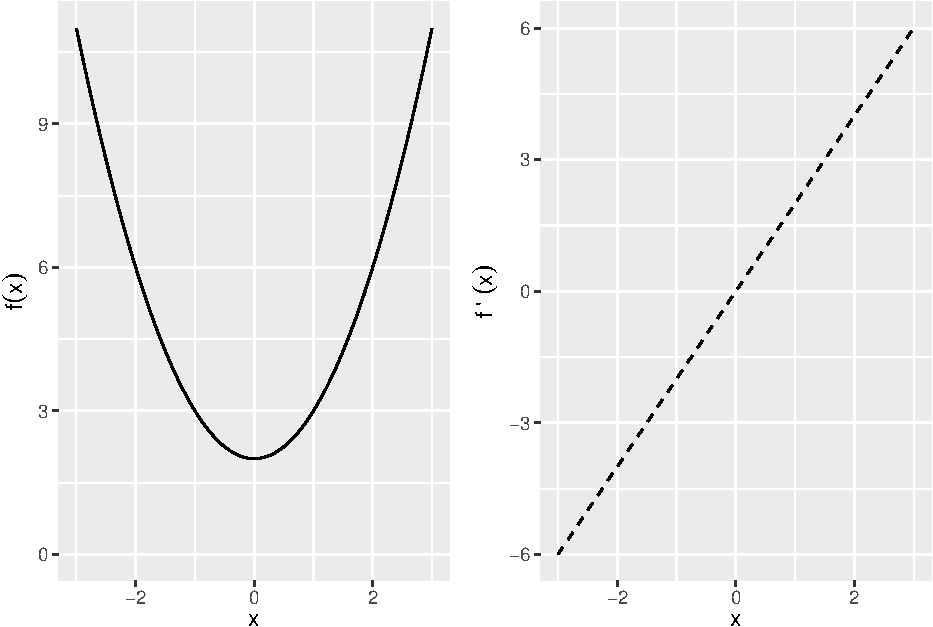
\includegraphics{figure-latex/unnamed-chunk-43-1.pdf}
\caption{\label{fig:unnamed-chunk-43}Maxima and Minima}
\end{figure}

\begin{exercise}[Plotting a mazimum and minimum]
\protect\hypertarget{exr:unnamed-chunk-44}{}\label{exr:unnamed-chunk-44}Plot \(f(x)=x^3+ x^2 + 2\), plot its derivative, and identifiy where the derivative is zero. Is there a maximum or minimum?
\end{exercise}

The second derivative \(f''(x)\) identifies whether the function \(f(x)\) at the point \(x\) is

\begin{enumerate}
\def\labelenumi{\arabic{enumi}.}
\tightlist
\item
  Concave down: \(f''(x)<0\)
\item
  Concave up: \(f''(x)>0\)
\end{enumerate}

\textbf{Maximum (Minimum)}: \(x_0\) is a \textbf{local maximum (minimum)} if \(f(x_0)>f(x)\) (\(f(x_0)<f(x))\) for all \(x\) within some open interval containing \(x_0\). \(x_0\) is a \textbf{global maximum (minimum)} if \(f(x_0)>f(x)\) (\(f(x_0)<f(x))\) for all \(x\) in the domain of \(f\).

Given the function \(f\) defined over domain \(D\), all of the following are defined as \textbf{critical points}:

\begin{enumerate}
\def\labelenumi{\arabic{enumi}.}
\tightlist
\item
  Any interior point of \(D\) where \(f'(x)=0\).
\item
  Any interior point of \(D\) where \(f'(x)\) does not exist.
\item
  Any endpoint that is in \(D\).
\end{enumerate}

The maxima and minima will be a subset of the critical points.

\textbf{Second Derivative Test of Maxima/Minima}: We can use the second derivative to tell us whether a point is a maximum or minimum of \(f(x)\).

\begin{enumerate}
\def\labelenumi{\arabic{enumi}.}
\tightlist
\item
  Local Maximum: \(f'(x)=0\) and \(f''(x)<0\)
\item
  Local Minimum: \(f'(x)=0\) and \(f''(x)>0\)
\item
  Need more info: \(f'(x)=0\) and \(f''(x)=0\)
\end{enumerate}

\textbf{Global Maxima and Minima} Sometimes no global max or min exists --- e.g., \(f(x)\) not bounded above or below. However, there are three situations where we can fairly easily identify global max or min.

\begin{enumerate}
\def\labelenumi{\arabic{enumi}.}
\tightlist
\item
  \textbf{Functions with only one critical point.} If \(x_0\) is a local max or min of \(f\) and it is the only critical point, then it is the global max or min.
\item
  \textbf{Globally concave up or concave down functions.} If \(f''(x)\) is never zero, then there is at most one critical point. That critical point is a global maximum if \(f''<0\) and a global minimum if \(f''>0\).
\item
  \textbf{Functions over closed and bounded intervals} must have both a global maximum and a global minimum.
\end{enumerate}

\begin{example}[Maxima and Minima by drawing]
\protect\hypertarget{exm:unnamed-chunk-46}{}\label{exm:unnamed-chunk-46}

Find any critical points and identify whether they are a max, min, or saddle point:

\begin{enumerate}
\def\labelenumi{\arabic{enumi}.}
\tightlist
\item
  \(f(x)=x^2+2\)
\item
  \(f(x)=x^3+2\)
\item
  \(f(x)=|x^2-1|\), \(x\in [-2,2]\)
\end{enumerate}

\end{example}

\hypertarget{concavity-of-a-function}{%
\section{Concavity of a Function}\label{concavity-of-a-function}}

Concavity helps identify the curvature of a function, \(f(x)\), in 2 dimensional space.

\begin{definition}[Concave Function]
\protect\hypertarget{def:unnamed-chunk-47}{}\label{def:unnamed-chunk-47}A function \(f\) is strictly concave over the set S \underline{if} \(\forall x_1,x_2 \in S\) and \(\forall a \in (0,1)\), \[f(ax_1 + (1-a)x_2) > af(x_1) + (1-a)f(x_2)\]
\textit{Any} line connecting two points on a concave function will lie \textit{below} the function.
\end{definition}

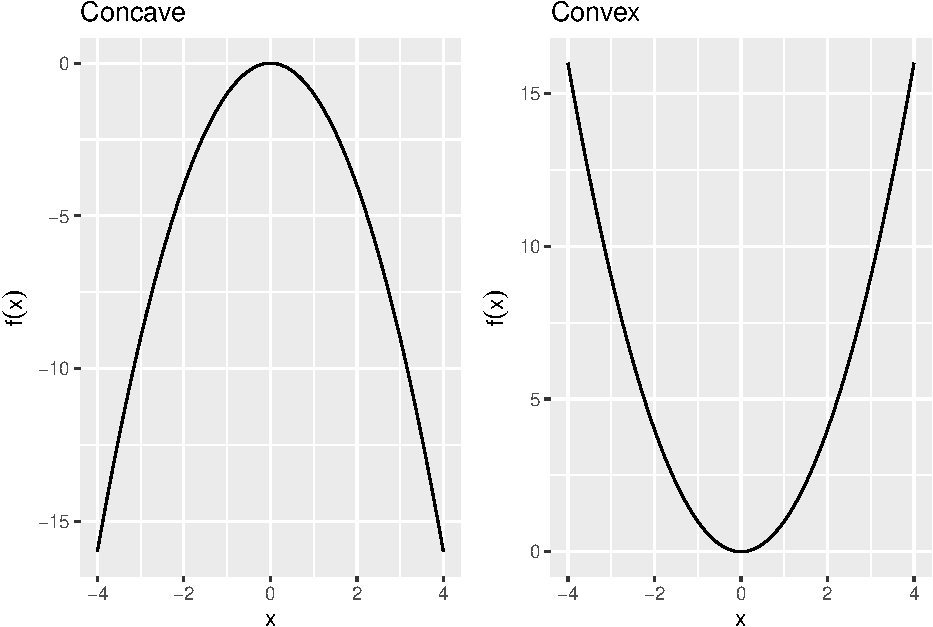
\includegraphics{figure-latex/unnamed-chunk-48-1.pdf}

\begin{definition}[Convex Function]
\protect\hypertarget{def:unnamed-chunk-49}{}\label{def:unnamed-chunk-49}Convex: A function f is strictly convex over the set S \underline{if} \(\forall x_1,x_2 \in S\) and \(\forall a \in (0,1)\), \[f(ax_1 + (1-a)x_2) < af(x_1) + (1-a)f(x_2)\]

Any line connecting two points on a convex function will lie above the function.
\end{definition}

\begin{comment}
  \parbox{2in}{\includegraphics[scale=.4]{Convex.pdf}}
\end{comment}

Sometimes, concavity and convexity are strict of a requirement. For most purposes of getting solutions, what we call quasi-concavity is enough.

\begin{definition}[Quasiconcave Function]
\protect\hypertarget{def:unnamed-chunk-50}{}\label{def:unnamed-chunk-50}A function f is quasiconcave over the set S if \(\forall x_1,x_2 \in S\) and \(\forall a \in (0,1)\), \[f(ax_1 + (1-a)x_2) \ge \min(f(x_1),f(x_2))\]

No matter what two points you select, the \textit{lowest} valued point will always be an end point.
\end{definition}

\begin{comment}
  \parbox{2in}{\includegraphics[scale=.4]{Quasiconcave.pdf}}
\end{comment}

\begin{definition}[Quasiconvex]
\protect\hypertarget{def:unnamed-chunk-51}{}\label{def:unnamed-chunk-51}A function f is quasiconvex over the set \(S\) if \(\forall x_1,x_2 \in S\) and \(\forall a \in (0,1)\), \[f(ax_1 + (1-a)x_2) \le \max(f(x_1),f(x_2))\]
No matter what two points you select, the \textit{highest} valued point will always be an end point.
\end{definition}

\begin{comment}
  \parbox{1.8in}{\includegraphics[scale=.4]{Quasiconvex.pdf}}
\end{comment}

\textbf{Second Derivative Test of Concavity}: The second derivative can be used to understand concavity.

If
\[\begin{array}{lll}
f''(x) < 0 & \Rightarrow & \text{Concave}\\
f''(x) > 0 & \Rightarrow & \text{Convex}
\end{array}\]

\hypertarget{quadratic-forms}{%
\subsection*{Quadratic Forms}\label{quadratic-forms}}
\addcontentsline{toc}{subsection}{Quadratic Forms}

Quadratic forms is shorthand for a way to summarize a function. This is important for finding concavity because

\begin{enumerate}
\def\labelenumi{\arabic{enumi}.}
\tightlist
\item
  Approximates local curvature around a point --- e.g., used to
  identify max vs min vs saddle point.
\item
  They are simple to express even in \(n\) dimensions:
\item
  Have a matrix representation.
\end{enumerate}

\textbf{Quadratic Form}: A polynomial where each term is a monomial
of degree 2 in any number of variables:

\begin{align*}
\text{One variable: }& Q(x_1) = a_{11}x_1^2\\
\text{Two variables: }& Q(x_1,x_2) = a_{11}x_1^2 + a_{12}x_1x_2 + a_{22}x_2^2\\
\text{N variables: }& Q(x_1,\cdots,x_n)=\sum\limits_{i\le j} a_{ij}x_i x_j
\end{align*}

which can be written in matrix terms:

One variable

\[Q(\mathbf{x}) = x_1^\top a_{11} x_1\]

N variables:
\begin{align*}
Q(\mathbf{x}) &=\begin{pmatrix} x_1 & x_2 & \cdots & x_n \end{pmatrix}\begin{pmatrix}
a_{11}&\frac{1}{2}a_{12}&\cdots&\frac{1}{2}a_{1n}\\
\frac{1}{2}a_{12}&a_{22}&\cdots&\frac{1}{2}a_{2n}\\
\vdots&\vdots&\ddots&\vdots\\
\frac{1}{2}a_{1n}&\frac{1}{2}a_{2n}&\cdots&a_{nn}
\end{pmatrix}
\begin{pmatrix} x_1\\x_2\\\vdots\\x_n\end{pmatrix}\\
&= \mathbf{x}^\top\mathbf{Ax}
\end{align*}

For example, the Quadratic on \(\mathbf{R}^2\):
\begin{align*}
  Q(x_1,x_2)&=\begin{pmatrix} x_1& x_2 \end{pmatrix} \begin{pmatrix} a_{11}&\frac{1}{2} a_{12}\\
  \frac{1}{2}a_{12}&a_{22}\end{pmatrix} \begin{pmatrix} x_1\\x_2 \end{pmatrix} \\
  &= a_{11}x_1^2 + a_{12}x_1x_2 + a_{22}x_2^2
\end{align*}

\hypertarget{definiteness-of-quadratic-forms}{%
\subsection*{Definiteness of Quadratic Forms}\label{definiteness-of-quadratic-forms}}
\addcontentsline{toc}{subsection}{Definiteness of Quadratic Forms}

When the function \(f(\mathbf{x})\) has more than two inputs, determining whether it has a maxima and minima (remember, functions may have many inputs but they have only one output) is a bit more tedious. Definiteness helps identify the curvature of a function, \(Q(\textbf{x})\), in n dimensional space.

\textbf{Definiteness}: By definition, a quadratic form always takes on the value of zero when \(x = 0\), \(Q(\textbf{x})=0\) at \(\textbf{x}=0\). The definiteness of the matrix \(\textbf{A}\) is determined by whether the
quadratic form \(Q(\textbf{x})=\textbf{x}^\top\textbf{A}\textbf{x}\) is greater than zero, less than
zero, or sometimes both over all \(\mathbf{x}\ne 0\).

\hypertarget{foc-and-soc}{%
\section{FOC and SOC}\label{foc-and-soc}}

We can see from a graphical representation that if a point is a local maxima or minima, it must meet certain conditions regarding its derivative. These are so commonly used that we refer these to ``First Order Conditions'' (FOCs) and ``Second Order Conditions'' (SOCs) in the economic tradition.

\hypertarget{first-order-conditions}{%
\subsection*{First Order Conditions}\label{first-order-conditions}}
\addcontentsline{toc}{subsection}{First Order Conditions}

When we examined functions of one variable \(x\), we found critical points by taking the first derivative, setting it to zero, and solving for \(x\). For functions of \(n\) variables, the critical points are found in much the same way, except now we set the partial derivatives equal to zero. Note: We will only consider critical points on the interior of a function's domain.

In a derivative, we only took the derivative with respect to one variable at a time. When we take the derivative separately with respect to all variables in the elements of \(\mathbf{x}\) and then express the result as a vector, we use the term Gradient and Hessian.

\begin{definition}[Gradient]
\protect\hypertarget{def:unnamed-chunk-52}{}\label{def:unnamed-chunk-52}Given a function \(f(\textbf{x})\) in \(n\) variables, the gradient \(\nabla f(\mathbf{x})\) (the greek letter nabla ) is a column vector, where the \(i\)th element is the partial derivative of \(f(\textbf{x})\) with respect to \(x_i\):

\[\nabla f(\mathbf{x}) = \begin{pmatrix}
\frac{\partial f(\mathbf{x})}{\partial x_1}\\ \frac{\partial f(\mathbf{x})}{\partial x_2}\\
  \vdots \\ \frac{\partial f(\mathbf{x})}{\partial x_n} \end{pmatrix}\]
\end{definition}

Before we know whether a point is a maxima or minima, if it meets the FOC it is a ``Critical Point''.

\begin{definition}[Critical Point]
\protect\hypertarget{def:unnamed-chunk-53}{}\label{def:unnamed-chunk-53}\(\mathbf{x}^*\) is a critical point if and only if \(\nabla f(\mathbf{x}^*)=0\). If the partial derivative of f(x) with respect to \(x^*\) is 0, then \(\mathbf{x}^*\) is a critical point. To solve for \(\mathbf{x}^*\), find the gradient, set each element equal to 0, and solve the system of equations. \[\mathbf{x}^* = \begin{pmatrix} x_1^*\\x_2^*\\ \vdots \\ x_n^*\end{pmatrix}\]
\end{definition}

\begin{example}
\protect\hypertarget{exm:unnamed-chunk-54}{}\label{exm:unnamed-chunk-54}Example: Given a function \(f(\mathbf{x})=(x_1-1)^2+x_2^2+1\), find the (1) Gradient and (2) Critical point of \(f(\mathbf{x})\).
\end{example}

\begin{solution}
Gradient

\begin{align*}
\nabla f(\mathbf{x}) &= \begin{pmatrix}\frac{\partial f(\mathbf{x})}{\partial x_1}\\ \frac{\partial f(\mathbf{x})}{\partial x_2} \end{pmatrix}\\
&= \begin{pmatrix} 2(x_1-1)\\ 2x_2 \end{pmatrix}
\end{align*}

Critical Point \(\mathbf{x}^* =\)

\begin{align*}
&\frac{\partial f(\mathbf{x})}{\partial x_1} = 2(x_1-1) = 0\\
&\Rightarrow x_1^* = 1\\
&\frac{\partial f(\mathbf{x})}{\partial x_2} = 2x_2 = 0\\
&\Rightarrow   x_2^* = 0\\
\end{align*}

So \[\mathbf{x}^* = (1,0)\]
\end{solution}

\hypertarget{second-order-conditions}{%
\subsection*{Second Order Conditions}\label{second-order-conditions}}
\addcontentsline{toc}{subsection}{Second Order Conditions}

When we found a critical point for a function of one variable, we used the second derivative as a indicator of the curvature at the point in order to determine whether the point was a min, max, or saddle (second derivative test of concavity). For functions of \(n\) variables, we use \emph{second order partial derivatives} as an indicator of curvature.

\begin{definition}[Hessian]
\protect\hypertarget{def:unnamed-chunk-56}{}\label{def:unnamed-chunk-56}Given a function \(f(\mathbf{x})\) in \(n\) variables, the hessian \(\mathbf{H(x)}\) is
an \(n\times n\) matrix, where the \((i,j)\)th element is the second order
partial derivative of \(f(\mathbf{x})\) with respect to \(x_i\) and \(x_j\):

\[\mathbf{H(x)}=\begin{pmatrix}
\frac{\partial^2 f(\mathbf{x})}{\partial x_1^2}&\frac{\partial^2f(\mathbf{x})}{\partial x_1 \partial x_2}&
\cdots & \frac{\partial^2 f(\mathbf{x})}{\partial x_1 \partial x_n}\\[9pt]
\frac{\partial^2 f(\mathbf{x})}{\partial x_2 \partial x_1}&\frac{\partial^2f(\mathbf{x})}{\partial x_2^2}&
\cdots & \frac{\partial^2 f(\mathbf{x})}{\partial x_2 \partial x_n}\\
\vdots & \vdots & \ddots & \vdots \\[3pt]
\frac{\partial^2 f(\mathbf{x})}{\partial x_n \partial x_1}&\frac{\partial^2f(\mathbf{x})}{\partial x_n \partial x_2}&
\cdots & \frac{\partial^2 f(\mathbf{x})}{\partial x_n^2}\end{pmatrix}\]
\end{definition}

Note that the hessian will be a symmetric matrix because \(\frac{\partial f(\mathbf{x})}{\partial x_1\partial x_2} = \frac{\partial f(\mathbf{x})}{\partial x_2\partial x_1}\).

Also note that given that \(f(\mathbf{x})\) is of quadratic form, each element of the hessian will be a constant.

These definitions will be employed when we determine the \textbf{Second Order Conditions} of a function:

Given a function \(f(\mathbf{x})\) and a point \(\mathbf{x}^*\) such that \(\nabla f(\mathbf{x}^*)=0\),

\begin{enumerate}
\def\labelenumi{\arabic{enumi}.}
\tightlist
\item
  Hessian is Positive Definite \(\quad \Longrightarrow \quad\) Strict Local Min
\item
  Hessian is Positive Semidefinite \(\forall \mathbf{x}\in B(\mathbf{x}^*,\epsilon)\)\} \(\quad \Longrightarrow \quad\) Local Min
\item
  Hessian is Negative Definite \(\quad \Longrightarrow \quad\) Strict Local Max
\item
  Hessian is Negative Semidefinite \(\forall \mathbf{x}\in B(\mathbf{x}^*,\epsilon)\)\} \(\quad \Longrightarrow \quad\) Local Max
\item
  Hessian is Indefinite \(\quad \Longrightarrow \quad\) Saddle Point
\end{enumerate}

\begin{example}[Max and min with two dimensions]
\protect\hypertarget{exm:unnamed-chunk-57}{}\label{exm:unnamed-chunk-57}We found that the only critical point of
\(f(\mathbf{x})=(x_1-1)^2+x_2^2+1\) is at \(\mathbf{x}^*=(1,0)\). Is it a min, max, or
saddle point?
\end{example}

\begin{solution}
The Hessian is
\begin{align*}
\mathbf{H(x)} &= \begin{pmatrix} 2&0\\0&2 \end{pmatrix}
\end{align*}
The Leading principal minors of the Hessian are \(M_1=2; M_2=4\). Now we consider Definiteness. Since both leading principal minors are positive, the Hessian is positive definite.

Maxima, Minima, or Saddle Point? Since the Hessian is positive definite and the gradient equals 0, \(x^\star = (1,0)\) is a strict local minimum.

Note: Alternate check of definiteness. Is \(\mathbf{H(x^*)} \geq \leq 0 \quad \forall \quad \mathbf{x}\ne 0\)

\begin{align*}
\mathbf{x}^\top H(\mathbf{x}^*) \mathbf{x} &= \begin{pmatrix} x_1 & x_2 \end{pmatrix}\\
&= \begin{pmatrix} 2&0\\0&2 \end{pmatrix}\\
\begin{pmatrix} x_1\\x_2\end{pmatrix} &= 2x_1^2+2x_2^2
\end{align*}

For any \(\mathbf{x}\ne 0\), \(2(x_1^2+x_2^2)>0\), so the Hessian is positive definite and \(\mathbf{x}^*\) is a strict local minimum.
\end{solution}

\hypertarget{definiteness-and-concavity}{%
\subsection*{Definiteness and Concavity}\label{definiteness-and-concavity}}
\addcontentsline{toc}{subsection}{Definiteness and Concavity}

Although definiteness helps us to understand the curvature of an n-dimensional function, it does not necessarily tell us whether the function is globally concave or convex.

We need to know whether a function is globally concave or convex to determine whether a critical point is a global min or max. We can use the definiteness of the Hessian to determine whether a function is globally concave or convex:

\begin{enumerate}
\def\labelenumi{\arabic{enumi}.}
\tightlist
\item
  Hessian is Positive Semidefinite \(\forall \mathbf{x}\)\} \(\quad \Longrightarrow \quad\) Globally Convex
\item
  Hessian is Negative Semidefinite \(\forall \mathbf{x}\)\} \(\quad \Longrightarrow \quad\) Globally Concave
\end{enumerate}

Notice that the definiteness conditions must be satisfied over the entire domain.

\hypertarget{global-maxima-and-minima}{%
\section{Global Maxima and Minima}\label{global-maxima-and-minima}}

\textbf{Global Max/Min Conditions}: Given a function \(f(\mathbf{x})\) and a point \(\mathbf{x}^*\) such that \(\nabla f(\mathbf{x}^*)=0\),

\begin{enumerate}
  \item \parbox[t]{2in}{$f(\mathbf{x})$ Globally Convex} $\quad
\Longrightarrow \quad$ Global Min
  \item \parbox[t]{2in}{$f(\mathbf{x})$ Globally Concave} $\quad
\Longrightarrow \quad$ Global Max
\end{enumerate}

Note that showing that \(\mathbf{H(x^*)}\) is negative semidefinite is
not enough to guarantee \(\mathbf{x}^*\) is a local max. However, showing that
\(\mathbf{H(x)}\) is negative semidefinite for all \(\mathbf{x}\) guarantees that \(x^*\)
is a global max. (The same goes for positive semidefinite and minima.)\textbackslash{}

Example: Take \(f_1(x)=x^4\) and \(f_2(x)=-x^4\). Both have \(x=0\) as
a critical point. Unfortunately, \(f''_1(0)=0\) and \(f''_2(0)=0\), so we
can't tell whether \(x=0\) is a min or max for either. However,
\(f''_1(x)=12x^2\) and \(f''_2(x)=-12x^2\). For all \(x\), \(f''_1(x)\ge 0\)
and \(f''_2(x)\le 0\) --- i.e., \(f_1(x)\) is globally convex and \(f_2(x)\)
is globally concave. So \(x=0\) is a global min of \(f_1(x)\) and a
global max of \(f_2(x)\).

\begin{exercise}
\protect\hypertarget{exr:unnamed-chunk-59}{}\label{exr:unnamed-chunk-59}Given \(f(\mathbf{x})=x_1^3-x_2^3+9x_1x_2\), find any maxima or minima.
\end{exercise}

\begin{enumerate}
  \item First order conditions.  
    \begin{enumerate}
    \item Gradient $\nabla f(\mathbf{x}) = $
        $$\phantom{\begin{pmatrix} \frac{\partial f}{\partial x_1} \\ 
        \frac{\partial f}{\partial x_2}\end{pmatrix} =
        \begin{pmatrix} 3x_1^2+9x_2 \\ -3x_2^2+9x_1 \end{pmatrix}}$$
    \item Critical Points $\mathbf{x^*} =$\\
        \phantom{Set the gradient equal to zero and solve for $x_1$ and 
        $x_2$.We have two equations and two unknowns.  Solving for $x_1$ 
        and $x_2$, we get two critical points:  $\mathbf{x}_1^*=(0,0)$ and
        $\mathbf{x}_2^*=(3,-3)$.}
        $$\phantom{3x_1^2 + 9x_2 = 0 \quad \Rightarrow \quad  9x_2 = 
        -3x_1^2 \quad \Rightarrow \quad  x_2 = -\frac{1}{3}x_1^2}$$
        $$\phantom{-3x_2^2 + 9x_1 = 0 \quad \Rightarrow \quad 
        -3(-\frac{1} {3}x_1^2)^2 + 9x_1 = 0}$$ 
        $$\phantom{\Rightarrow \quad -\frac{1}{3}x_1^4 
        + 9x_1 = 0 \quad \Rightarrow \quad x_1^3 = 27x_1 \quad 
        \Rightarrow \quad x_1 = 3}$$
        $$\phantom{3(3)^2 + 9x_2 = 0 \quad \Rightarrow \quad x_2 = -3}$$    
    \end{enumerate}       
 
  \item Second order conditions.  
    \begin{enumerate}
    \item Hessian $\mathbf{H(x)} = $
        $$\phantom{\begin{pmatrix} 6x_1&9\\9&-6x_2 \end{pmatrix}}$$
    \item Hessian $\mathbf{H(x_1^*)} = $
        $$\phantom{\begin{pmatrix} 0&9\\9&0\end{pmatrix}}$$
    \item Leading principal minors of $\mathbf{H(x_1^*)} = $
        $$\phantom{M_1=0; M_2=-81}$$\\
    \item Definiteness of $\mathbf{H(x_1^*)}$?\\
        \phantom{$\mathbf{H(x_1^*)}$ is indefinite}\\
    \item Maxima, Minima, or Saddle Point for $\mathbf{x_1^*}$?\\
        \phantom{Since $\mathbf{H(x_1^*)}$ is indefinite, $\mathbf{x}_1^*=(0,0)$ 
        is a saddle point.}\\
    \item Hessian $\mathbf{H(x_2^*)} = $
        $$\phantom{\begin{pmatrix} 18&9\\9&18\end{pmatrix}}$$
    \item Leading principal minors of $\mathbf{H(x_2^*)} = $
        $$\phantom{M_1=18; M_2=243}$$\\
    \item Definiteness of $\mathbf{H(x_2^*)}$?\\
        \phantom{$\mathbf{H(x_2^*)}$ is positive definite}\\
    \item Maxima, Minima, or Saddle Point for $\mathbf{x}_2^*$?\\
        \phantom{Since $\mathbf{H(x_2^*)}$ is positive definite, $\mathbf{x}_1^*=(3,-3)$ is a strict local minimum}\\
    \end{enumerate}   
    
  \item Global concavity/convexity.  
    \begin{enumerate}
    \item Is f(x) globally concave/convex?\\
        \phantom{No.    In evaluating the Hessians for $\mathbf{x}_1^*$ 
        and $\mathbf{x}_2^*$ we saw that the Hessian is not positive 
        semidefinite at x $=$ (0,0).}\\
    \item Are any $\mathbf{x^*}$ global minima or maxima?\\
        \phantom{No. Since the function is not globally concave/convex, 
        we can't infer that $\mathbf{x}_2^*=(3,-3)$ is a global minimum.  
        In fact, if we set $x_1=0$, the $f(\mathbf{x})=-x_2^3$, which will 
        go to $-\infty$ as $x_2\to \infty$.}\\
    \end{enumerate}       
\end{enumerate}

\hypertarget{constrained-optimization}{%
\section{Constrained Optimization}\label{constrained-optimization}}

We have already looked at optimizing a function in one or more dimensions over the whole domain of the function. Often, however, we want to find the maximum or minimum of a function over some restricted part of its domain.

ex: Maximizing utility subject to a budget constraint

\begin{figure}
\centering
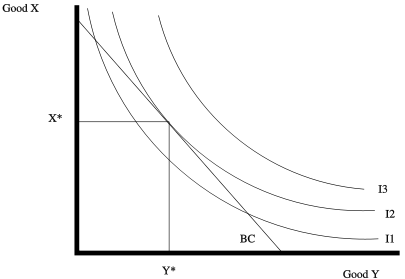
\includegraphics{figure-latex/constraint.png}
\caption{A typical Utility Function with a Budget Constraint}
\end{figure}

\textbf{Types of Constraints}: For a function \(f(x_1, \dots, x_n)\), there are two types of constraints that can be imposed:

\begin{enumerate}
\item \textbf{Equality constraints:} constraints of the form $c(x_1,\dots, x_n) = r$.
Budget constraints are the classic example of equality constraints in social science.
\item \textbf{Inequality constraints:} constraints of the form $c(x_1, \dots, x_n) \leq r$.  These might arise from non-negativity constraints or other threshold effects.
\end{enumerate}

In any constrained optimization problem, the constrained maximum will always be less than or equal to the unconstrained maximum. If the constrained maximum is less than the unconstrained maximum, then the constraint is binding. Essentially, this means that you can treat your constraint as an equality constraint rather than an inequality constraint.

For example, the budget constraint binds when you spend your entire budget. This generally happens because we believe that utility is strictly increasing in consumption, i.e.~you always want more so you spend everything you have.

Any number of constraints can be placed on an optimization problem. When working with multiple constraints, always make sure that the set of constraints are not pathological; it must be possible for all of the constraints to be satisfied simultaneously.

\textbf{Set-up for Constrained Optimization:}
\[\max_{x_1,x_2} f(x_1,x_2) \text{ s.t. } c(x_1,x_2)\]
\[\min_{x_1,x_2} f(x_1,x_2) \text{ s.t. } c(x_1,x_2)\]
This tells us to maximize/minimize our function, \(f(x_1,x_2)\), with respect to the choice variables, \(x_1,x_2\), subject to the constraint.

Example:
\[\max_{x_1,x_2} f(x_1, x_2) = -(x_1^2 + 2x_2^2) \text{ s.t. }x_1 + x_2 = 4\]
It is easy to see that the \textit{unconstrained} maximum occurs at \((x_1, x_2) = (0,0)\), but that does not satisfy the constraint. How should we proceed?

\hypertarget{equality-constraints}{%
\subsection*{Equality Constraints}\label{equality-constraints}}
\addcontentsline{toc}{subsection}{Equality Constraints}

Equality constraints are the easiest to deal with because we know that the maximum or minimum has to lie on the (intersection of the) constraint(s).

The trick is to change the problem from a constrained optimization problem in \(n\) variables to an unconstrained optimization problem in \(n + k\) variables, adding \emph{one} variable for \emph{each} equality constraint. We do this using a lagrangian multiplier.

\textbf{Lagrangian function}: The Lagrangian function allows us to combine the function we want to optimize and the constraint function into a single function. Once we have this single function, we can proceed as if this were an \emph{unconstrained} optimization problem.

For each constraint, we must include a \textbf{Lagrange multiplier} (\(\lambda_i\)) as an additional variable in the analysis. These terms are the link between the constraint and the Lagrangian function.

Given a \emph{two dimensional} set-up:
\[\max_{x_1,x_2}/\min_{x_1,x_2} f(x_1,x_2) \text{ s.t. } c(x_1,x_2) = a\]

We define the Lagrangian function \(L(x_1,x_2,\lambda_1)\) as follows:
\[L(x_1,x_2,\lambda_1) = f(x_1,x_2) - \lambda_1 (c(x_1,x_2) - a)\]

More generally, in \emph{n dimensions}:
\[ L(x_1, \dots, x_n, \lambda_1, \dots, \lambda_k) = f(x_1, \dots, x_n) - \sum_{i=1}^k\lambda_i(c_i(x_1,\dots, x_n) - r_i)\]

\textbf{Getting the sign right:} Note that above we subtract the lagrangian term \emph{and} we subtract the constraint constant from the constraint function. Occasionally, you may see the following alternative form of the Lagrangian, which is \emph{equivalent}:
\[ L(x_1, \dots, x_n, \lambda_1, \dots, \lambda_k) = f(x_1, \dots, x_n) + \sum_{i=1}^k\lambda_i(r_i - c_i(x_1,\dots, x_n))\]
Here we add the lagrangian term \emph{and} we subtract the constraining function from the constraint constant.

\textbf{Using the Lagrangian to Find the Critical Points}: To find the critical points, we take the partial derivatives of lagrangian function, \(L(x_1, \dots, x_n, \lambda_1, \dots, \lambda_k)\), with respect to each of its variables (all choice variables \(\mathbf{x}\) \emph{and} all lagrangian multipliers \(\mathbf{\lambda}\)). At a critical point, each of these partial derivatives must be equal to zero, so we obtain a system of \(n + k\) equations in \(n + k\) unknowns:

\begin{align*}
\frac{\partial L}{\partial x_1} &= \frac{\partial f}{\partial x_1} - \sum_{i = 1}^k\lambda_i\frac{\partial c_i}{\partial x_1} = 0\\
 \vdots &= \vdots \nonumber \\ 
\frac{\partial L}{\partial x_n}  &= \frac{\partial f}{\partial x_n} - \sum_{i = 1}^k\lambda_i\frac{\partial c_i}{\partial x_n} = 0\\
\frac{\partial L}{\partial \lambda_1} &= c_1(x_i, \dots, x_n) - r_1 =  0\\
 \vdots &= \vdots \nonumber \\
\frac{\partial L}{\partial \lambda_k} &= c_k(x_i, \dots, x_n) - r_k = 0
\end{align*}

We can then solve this system of equations, because there are \(n+k\) equations and \(n+k\) unknowns, to calculate the critical point \((x_1^*,\dots,x_n^*,\lambda_1^*,\dots,\lambda_k^*)\).

\textbf{Second-order Conditions and Unconstrained Optimization:} There may be more than one critical point, i.e.~we need to verify that the critical point we find is a maximum/minimum. Similar to unconstrained optimization, we can do this by checking the second-order conditions.

\begin{example}[Constrained optimization with two goods and a budget constraint]
\protect\hypertarget{exm:unnamed-chunk-60}{}\label{exm:unnamed-chunk-60}Find the constrained optimization of
\[\max_{x_1,x_2} f(x) = -(x_1^2 + 2x_2^2) \text{ s.t. } x_1 + x_2 = 4\]
\end{example}

\begin{solution}

\begin{enumerate}
\def\labelenumi{\arabic{enumi}.}
\tightlist
\item
  Begin by writing the Lagrangian:
  \[L(x_1, x_2, \lambda) =  -(x_1^2 + 2x_2^2) - \lambda(x_1 + x_2 - 4)\]
\item
  Take the partial derivatives and set equal to zero:
\end{enumerate}

\begin{align*}
\frac{\partial L}{\partial x_1} = -2x_1 - \lambda \quad \quad \quad &= 0\\
\frac{\partial L}{\partial x_2}  = -4x_2 - \lambda \quad \quad \quad &= 0\\
\frac{\partial L}{\partial \lambda} = -(x_1 + x_2 - 4) \quad & = & 0\\
\end{align*}

\begin{enumerate}
\def\labelenumi{\arabic{enumi}.}
\setcounter{enumi}{2}
\item
  Solve the system of equations: Using the first two partials, we see that \(\lambda = -2x_1\) and \(\lambda = -4x_2\)
  Set these equal to see that \(x_1 = 2x_2\).
  Using the third partial and the above equality, \(4 = 2x_2 + x_2\) from which we get \[x_2^* = 4/3, x_1^* = 8/3, \lambda = -16/3\]
\item
  Therefore, the only critical point is \(x_1^* = \frac{8}{3}\) and \(x_2^* = \frac{4}{3}\)
\item
  This gives \(f(\frac{8}{3}, \frac{4}{3}) = -\frac{96}{9}\), which is less than the unconstrained optimum \(f(0,0) = 0\)
\end{enumerate}

\end{solution}

Notice that when we take the partial derivative of L with respect to the Lagrangian multiplier and set it equal to 0, we return exactly our constraint! This is why signs matter.

\hypertarget{inequality-constraints}{%
\section{Inequality Constraints}\label{inequality-constraints}}

Inequality constraints define the boundary of a region over which we seek to optimize the function. This makes inequality constraints more challenging because we do not know if the maximum/minimum lies along one of the constraints (the constraint binds) or in the interior of the region.

We must introduce more variables in order to turn the problem into an unconstrained optimization.

\textbf{Slack:} For each inequality constraint \(c_i(x_1, \dots, x_n) \leq a_i\), we define a slack variable \(s_i^2\) for which the expression \(c_i(x_1, \dots, x_n) \leq a_i - s_i^2\) would hold with equality. These slack variables capture how close the constraint comes to binding. We use \(s^2\) rather than \(s\) to ensure that the slack is positive.

Slack is just a way to transform our constraints.

Given a two-dimensional set-up and these edited constraints:
\[\max_{x_1,x_2}/\min_{x_1,x_2} f(x_1,x_2) \text{ s.t. } c(x_1,x_2) \le a_1\]

Adding in Slack:
\[\max_{x_1,x_2}/\min_{x_1,x_2} f(x_1,x_2) \text{ s.t. } c(x_1,x_2) \le a_1 - s_1^2\]

We define the Lagrangian function \(L(x_1,x_2,\lambda_1,s_1)\) as follows:
\[L(x_1,x_2,\lambda_1,s_1) = f(x_1,x_2) - \lambda_1 ( c(x_1,x_2) + s_1^2 - a_1)\]

More generally, in n dimensions:
\[ L(x_1, \dots, x_n, \lambda_1, \dots, \lambda_k, s_1, \dots, s_k) = f(x_1, \dots, x_n) - \sum_{i = 1}^k \lambda_i(c_i(x_1,\dots, x_n) + s_i^2 - a_i)\]

\textbf{Finding the Critical Points}: To find the critical points, we take the partial derivatives of the lagrangian function, \(L(x_1,\dots,x_n,\lambda_1,\dots,\lambda_k,s_1,\dots,s_k)\), with respect to each of its variables (all choice variables \(x\), all lagrangian multipliers \(\lambda\), and all slack variables \(s\)). At a critical point, \emph{each} of these partial derivatives must be equal to zero, so we obtain a system of \(n + 2k\) equations in \(n + 2k\) unknowns:

\begin{align*}
\frac{\partial L}{\partial x_1} &= \frac{\partial f}{\partial x_1} - \sum_{i = 1}^k\lambda_i\frac{\partial c_i}{\partial x_1} = 0\\
 \vdots & =  \vdots  \\
\frac{\partial L}{\partial x_n}  &= \frac{\partial f}{\partial x_n} - \sum_{i = 1}^k\lambda_i\frac{\partial c_i}{\partial x_n} = 0\\
\frac{\partial L}{\partial \lambda_1} &= c_1(x_i, \dots, x_n) + s_1^2 - b_1 = 0\\
 \vdots & = \vdots \\
\frac{\partial L}{\partial \lambda_k} &= c_k(x_i, \dots, x_n) + s_k^2 - b_k = 0\\
\frac{\partial L}{\partial s_1} &= 2s_1\lambda_1 = 0\\
 \vdots =\vdots \\
\frac{\partial L}{\partial s_k} &= 2s_k\lambda_k = 0
\end{align*}

\textbf{Complementary slackness conditions}: The last set of first order conditions of the form \(2s_i\lambda_i = 0\) (the partials taken with respect to the slack variables) are known as complementary slackness conditions. These conditions can be satisfied one of three ways:

\begin{enumerate}
\def\labelenumi{\arabic{enumi}.}
\tightlist
\item
  \(\lambda_i = 0\) and \(s_i \neq 0\): This implies that the slack is positive and thus \emph{the constraint does not bind}.
\item
  \(\lambda_i \neq 0\) and \(s_i = 0\): This implies that there is no slack in the constraint and \emph{the constraint does bind}.
\item
  \(\lambda_i = 0\) and \(s_i = 0\): In this case, there is no slack but the \emph{constraint binds trivially}, without changing the optimum.
\end{enumerate}

Example: Find the critical points for the following constrained optimization:
\[\max_{x_1,x_2} f(x) = -(x_1^2 + 2x_2^2) \text{ s.t. } x_1 + x_2 \le 4\]

\begin{enumerate}
\def\labelenumi{\arabic{enumi}.}
\item
  Rewrite with the slack variables:
  \[\max_{x_1,x_2} f(x) = -(x_1^2 + 2x_2^2) \text{ s.t. } x_1 + x_2 \le 4 - s_1^2\]
\item
  Write the Lagrangian:
  \[L(x_1,x_2,\lambda_1,s_1) = -(x_1^2 + 2x_2^2) - \lambda_1 (x_1 + x_2 + s_1^2 - 4)\]
\item
  Take the partial derivatives and set equal to 0:
\end{enumerate}

\begin{align*}
\frac{\partial L}{\partial x_1} = -2x_1 - \lambda_1  &= 0\\
\frac{\partial L}{\partial x_2}  = -4x_2 - \lambda_1 &=  0\\
\frac{\partial L}{\partial \lambda_1} = -(x_1 + x_2 + s_1^2 - 4)&= 0\\
\frac{\partial L}{\partial s_1} = -2s_1\lambda_1 &= 0\\
\end{align*}

\begin{enumerate}
\def\labelenumi{\arabic{enumi}.}
\setcounter{enumi}{3}
\tightlist
\item
  Consider all ways that the complementary slackness conditions are solved:

  \begin{center}
  \begin{tabular}{|l|cccc|c|}
  \hline
  Hypothesis & $s_1$ & $\lambda_1$ & $x_1$ & $x_2$ & $f(x_1, x_2)$\\
  \hline
  $s_1 = 0$ $\lambda_1 = 0$ & \multicolumn{4}{l|}{No solution} & \\
  $s_1 \neq 0$ $\lambda_1 = 0$ & 2 & 0 & 0 & 0  & 0\\
  $s_1 = 0$ $\lambda_1 \neq 0$ & 0 & $\frac{-16}{3}$ & $\frac{8}{3}$ & $\frac{4}{3}$ & $-\frac{32}{3}$\\
  $s_1 \neq 0$ $\lambda_1 \neq 0$ & \multicolumn{4}{l|}{No solution} &\\
  \hline
  \end{tabular}
  \end{center}
\end{enumerate}

This shows that there are two critical points: \((0,0)\) and \((\frac{8}{3},\frac{4}{3})\).

\begin{enumerate}
\def\labelenumi{\arabic{enumi}.}
\setcounter{enumi}{4}
\tightlist
\item
  Find maximum:
  Looking at the values of \(f(x_1,x_2)\) at the critical points, we see that \(f(x_1,x_2)\) is maximized at \(x_1^* = 0\) and \(x_2^*=0\).
\end{enumerate}

\begin{exercise}
\protect\hypertarget{exr:unnamed-chunk-62}{}\label{exr:unnamed-chunk-62}Example: Find the critical points for the following constrained optimization:
\[\max_{x_1,x_2} f(x) = -(x_1^2 + 2x_2^2) \text{ s.t. } 
\begin{array}{l}
x_1 + x_2 \le 4\\
x_1 \ge 0\\
x_2 \ge 0
\end{array}\]
\end{exercise}

\begin{enumerate}
\def\labelenumi{\arabic{enumi}.}
\item
  Rewrite with the slack variables:
  \[\phantom{max_{x_1,x_2} f(x) = -(x_1^2 + 2x_2^2) \text{ s.t. } 
  \begin{array}{l}
  x_1 + x_2 \le 4 - s_1^2\\
  -x_1 \le 0 - s_2^2\\
  -x_2 \le 0 - s_3^2
  \end{array}}\]
\item
  Write the Lagrangian:
  \[\phantom{L(x_1, x_2, \lambda_1, \lambda_2, \lambda_3, s_1, s_2, s_3) =  -(x_1^2 + 2x_2^2) - \lambda_1(x_1 + x_2 + s_1^2  - 4) - \lambda_2(-x_1 + s_2^2) - \lambda_3(-x_2 + s_3^2)}\]
\item
  Take the partial derivatives and set equal to zero:
\end{enumerate}

\phantom{
$\frac{\partial L}{\partial x_1} = -2x_1 - \lambda_1 + \lambda_2  =  0$\\
$\frac{\partial L}{\partial x_2}  = -4x_2 - \lambda_1 + \lambda_3  =   0$\\
$\frac{\partial L}{\partial \lambda_1} = -(x_1 + x_2 + s_1^2 - 4) =  0$\\
$\frac{\partial L}{\partial \lambda_2} = -(-x_1 + s_2^2)  =  0$\\
$\frac{\partial L}{\partial \lambda_3} = -(-x_2 + s_3^2)  =  0$\\
$\frac{\partial L}{\partial s_1} = 2s_1\lambda_1  =  0$\\
$\frac{\partial L}{\partial s_2} = 2s_2\lambda_2  =  0$\\
$\frac{\partial L}{\partial s_3} = 2s_3\lambda_3  =  0$}

\begin{enumerate}
\def\labelenumi{\arabic{enumi}.}
\setcounter{enumi}{3}
\tightlist
\item
  Consider all ways that the complementary slackness conditions are solved:

  \begin{center}
  \begin{tabular}{|l|cccccccc|c|}
  \hline
  Hypothesis & $s_1$ & $s_2$ & $s_3$ & $\lambda_1$ & $\lambda_2$ & $\lambda_3$ & $x_1$ & $x_2$ & $f(x_1, x_2)$\\
  \hline
  $s_1 = s_2 = s_3 = 0$ & \multicolumn{8}{l|}{\phantom{No solution}} & \\
  $s_1 \neq 0, s_2 = s_3 = 0$ & \phantom{2} & \phantom{0} & \phantom{0} & \phantom{0} & \phantom{0} & \phantom{0} & \phantom{0} & \phantom{0} & \phantom{0}\\
  $s_2 \neq 0, s_1 = s_3 = 0$ & \phantom{0} & \phantom{2} & \phantom{0} & \phantom{-8} & \phantom{0} & \phantom{-8} & \phantom{4} & \phantom{0} & \phantom{-16}\\
  $s_3 \neq 0, s_1 = s_2 = 0$ & \phantom{0} & \phantom{0} & \phantom{2} & \phantom{-16} & \phantom{-16} & \phantom{0} & \phantom{0} & \phantom{4} & \phantom{-32}\\
  $s_1 \neq 0, s_2 \neq 0, s_3 = 0$ &\multicolumn{8}{l|}{\phantom{No solution}} & \\
  $s_1 \neq 0, s_3 \neq 0, s_2 = 0$ &\multicolumn{8}{l|}{\phantom{No solution}} & \\
  $s_2 \neq 0, s_3 \neq 0, s_1 = 0$ &\phantom{0} & \phantom{$\sqrt{\frac{8}{3}}$} & \phantom{$\sqrt{\frac{4}{3}}$} & \phantom{$-\frac{16}{3}$} & \phantom{0} & \phantom{0} & \phantom{$\frac{8}{3}$}& \phantom{$\frac{4}{3}$} & \phantom{$-\frac{32}{3}$}\\
  $s_1 \neq 0, s_2 \neq 0, s_3 \neq 0$ &\multicolumn{8}{l|}{\phantom{No solution}}& \\
  \hline
  \end{tabular}
  \end{center}
\end{enumerate}

\phantom{This shows that there are four critical points: $(0,0)$, $(4,0)$, $(0,4)$, and $(\frac{8}{3},\frac{4}{3})$}

\begin{enumerate}
\def\labelenumi{\arabic{enumi}.}
\setcounter{enumi}{4}
\tightlist
\item
  Find maximum: \phantom{Looking at the values of $f(x_1,x_2)$ at the critical points, we see that the constrained maximum is located at $(x_1, x_2) = (0,0)$, which is the same as the unconstrained max.  The constrained minimum is located at $(x_1, x_2) = (0,4)$, while there is no unconstrained minimum for this problem.}
\end{enumerate}

\hypertarget{kuhn-tucker-conditions}{%
\section{Kuhn-Tucker Conditions}\label{kuhn-tucker-conditions}}

As you can see, this can be a pain. When dealing explicitly with \emph{non-negativity constraints}, this process is simplified by using the Kuhn-Tucker method.

Because the problem of maximizing a function subject to inequality and non-negativity constraints arises frequently in economics, the \textbf{Kuhn-Tucker conditions} provides a method that often makes it easier to both calculate the critical points and identify points that are (local) maxima.

Given a \emph{two-dimensional set-up}:
\[\max_{x_1,x_2}/\min_{x_1,x_2} f(x_1,x_2) \text{ s.t. }
\begin{array}{l}
c(x_1,x_2) \le a_1\\
x_1 \ge 0 \\
gx_2 \ge 0
\end{array}\]

We define the Lagrangian function \(L(x_1,x_2,\lambda_1)\) the same as if we did not have the non-negativity constraints:
\[L(x_1,x_2,\lambda_2) = f(x_1,x_2) - \lambda_1(c(x_1,x_2) - a_1)\]

More generally, in n dimensions:
\[ L(x_1, \dots, x_n, \lambda_1, \dots, \lambda_k) = f(x_1, \dots, x_n) - \sum_{i=1}^k\lambda_i(c_i(x_1,\dots, x_n) - a_i)\]

\textbf{Kuhn-Tucker and Complementary Slackness Conditions}: To find the critical points, we first calculate the Kuhn-Tucker conditions by taking the partial derivatives of the lagrangian function, \(L(x_1,\dots,x_n,\lambda_1,\dots,\lambda_k)\), with respect to each of its variables (all choice variable s\(x\) and all lagrangian multipliers \(\lambda\)) and we calculate the \emph{complementary slackness conditions} by multiplying each partial derivative by its respective variable \emph{and} include non-negativity conditions for all variables (choice variables \(x\) and lagrangian multipliers \(\lambda\)).

\textbf{Kuhn-Tucker Conditions}

\begin{align*}
\frac{\partial L}{\partial x_1} \leq 0, & \dots, \frac{\partial L}{\partial x_n} \leq 0\\
\frac{\partial L}{\partial \lambda_1} \geq 0, & \dots, \frac{\partial L}{\partial \lambda_m} \geq 0
\end{align*}

\textbf{Complementary Slackness Conditions}

\begin{align*}
x_1\frac{\partial L}{\partial x_1} = 0, & \dots, x_n\frac{\partial L}{\partial x_n} = 0\\
\lambda_1\frac{\partial L}{\partial \lambda_1} = 0, & \dots, \lambda_m \frac{\partial L}{\partial \lambda_m} = 0
\end{align*}

\textbf{Non-negativity Conditions}
\begin{eqnarray*}
x_1 \geq 0 & \dots & x_n \geq 0\\
\lambda_1 \geq 0 & \dots & \lambda_m \geq 0
\end{eqnarray*}

Note that some of these conditions are set equal to 0, while others are set as inequalities!

Note also that to minimize the function \(f(x_1, \dots, x_n)\), the simplest thing to do is maximize the function \(-f(x_1, \dots, x_n)\); all of the conditions remain the same after reformulating as a maximization problem.

There are additional assumptions (notably, f(x) is quasi-concave and the constraints are convex) that are sufficient to ensure that a point satisfying the Kuhn-Tucker conditions is a global max; if these assumptions do not hold, you may have to check more than one point.

\textbf{Finding the Critical Points with Kuhn-Tucker Conditions}: Given the above conditions, to find the critical points we solve the above system of equations. To do so, we must check \textit{all} border and interior solutions to see if they satisfy the above conditions.

In a two-dimensional set-up, this means we must check the following cases:

\begin{enumerate}
\def\labelenumi{\arabic{enumi}.}
\tightlist
\item
  \(x_1 = 0, x_2 = 0\) Border Solution
\item
  \(x_1 = 0, x_2 \neq 0\) Border Solution
\item
  \(x_1 \neq 0, x_2 = 0\) Border Solution
\item
  \(x_1 \neq 0, x_2 \neq 0\) Interior Solution
\end{enumerate}

\begin{example}[Kuhn-Tucker with two variables]
\protect\hypertarget{exm:unnamed-chunk-63}{}\label{exm:unnamed-chunk-63}Solve the following optimization problem with inequality constraints
\[\max_{x_1,x_2} f(x) = -(x_1^2 + 2x_2^2)\]

\begin{align*}
\text{ s.t. } 
\begin{cases}
&x_1 + x_2 *\le 4\\
&x_1 *\ge 0\\
&x_2 *\ge 0
\end{cases}
\end{align*}
\end{example}

\begin{enumerate}
\def\labelenumi{\arabic{enumi}.}
\item
  Write the Lagrangian:
  \[L(x_1, x_2, \lambda) =  -(x_1^2 + 2x_2^2) - \lambda(x_1 + x_2 - 4)\]
\item
  Find the First Order Conditions:
\end{enumerate}

Kuhn-Tucker Conditions
\begin{align*}
\frac{\partial L}{\partial x_1} = -2x_1 - \lambda  &\leq 0\\
\frac{\partial L}{\partial x_2}  = -4x_2 - \lambda & \leq  0\\
\frac{\partial L}{\partial \lambda} = -(x_1 + x_2 - 4)& \geq 0
\end{align*}

Complementary Slackness Conditions
\begin{align*}
x_1\frac{\partial L}{\partial x_2} = x_1(-2x_1 - \lambda)  &= 0\\
x_2\frac{\partial L}{\partial x_2} = x_2(-4x_2 - \lambda)  &= 0\\
\lambda\frac{\partial L}{\partial \lambda} = -\lambda(x_1 + x_2 - 4)&= 0
\end{align*}

Non-negativity Conditions
\begin{align*}
x_1 & \geq  0\\
x_2 & \geq 0\\
\lambda & \geq 0
\end{align*}

\begin{enumerate}
\def\labelenumi{\arabic{enumi}.}
\setcounter{enumi}{2}
\tightlist
\item
  Consider all border and interior cases:

  \begin{center}
  \begin{tabular}{|l|ccc|c|}
  \hline
  Hypothesis  & $\lambda$& $x_1$ & $x_2$ & $f(x_1, x_2)$\\
  \hline
  $x_1 = 0, x_2 = 0$  &0 & 0 & 0 & 0\\
  $x_1 = 0, x_2 \neq 0$  &-16 & 0 & 4 & -32\\
  $x_1 \neq 0, x_2 = 0$  &-8 & 4 & 0 & -16\\
  $x_1 \neq 0, x_2 \neq 0$ & $-\frac{16}{3}$ & $\frac{8}{3}$ & $\frac{4}{3}$ & $-\frac{32}{3}$\\
  \hline
  \end{tabular}
  \end{center}
\item
  Find Maximum:
  Three of the critical points violate the requirement that \(\lambda \geq 0\), so the point \((0,0,0)\) is the maximum.
\end{enumerate}

\begin{exercise}[Kuhn-Tucker with logs]
\protect\hypertarget{exr:unnamed-chunk-64}{}\label{exr:unnamed-chunk-64}Solve the constrained optimization problem,

\[\max_{x_1,x_2} f(x) = \frac{1}{3}\log (x_1 + 1) + \frac{2}{3}\log (x_2 + 1) \text{ s.t. }  
\begin{array}{l}
x_1 + 2x_2 \leq 4\\
     x_1 \geq 0\\
    x_2 \geq 0
\end{array}\]
\end{exercise}

\begin{enumerate}
\item Write the Lagrangian:
$$\phantom{L(x_1, x_2, \lambda) =  \frac{1}{3}\log(x_1+1) + \frac{2}{3}\log(x_2+1) - \lambda(x_1 + 2x_2 - 4)}$$

\item Find the First Order Conditions:\\
Kuhn-Tucker Conditions\\
\phantom{$\frac{\partial L}{\partial x_1} = \frac{1}{3(x_1+1)} - \lambda   \leq  0$\\
$\frac{\partial L}{\partial x_2}  = \frac{2}{3(x_2+1)} - \lambda  \leq   0$\\
$\frac{\partial L}{\partial \lambda} = -(x_1 + 2x_2 - 4) \geq  0$}\\
\item[]
\item[]
\item[]
\item[]
\item[]
\item[]
\item[]
\item[]
 
Complementary Slackness Conditions\\
\phantom{$x_1\frac{\partial L}{\partial x_2} = x_1(\frac{1}{3(x_1+1)} - \lambda)  =  0$\\
$x_2\frac{\partial L}{\partial x_2} = x_2(\frac{2}{3(x_2+1)} - \lambda)   =  0$\\
$\lambda\frac{\partial L}{\partial \lambda} = -\lambda(x_1 + 2x_2 - 4) =  0$}\\
\item[]
\item[]
\item[]
\item[]
\item[]
\item[]
\item[]
\item[]
\item[]

Non-negativity Conditions\\
\phantom{$x_1  \geq  0$\\
$x_2  \geq  0$\\
$\lambda  \geq  $0}\\
\item[]
\item[]
\item[]

\item Consider all border and interior cases:
\begin{center}
\begin{tabular}{|l|ccc|c|}
\hline
Hypothesis  & $\lambda$& $x_1$ & $x_2$ & $f(x_1, x_2)$\\
\hline
$x_1 = 0, x_2 = 0$  &\multicolumn{3}{l|}{\phantom{No Solution}}& \\
$x_1 = 0, x_2 \neq 0$  &\multicolumn{3}{l|}{\phantom{No Solution}}& \\
$x_1 \neq 0, x_2 = 0$  & \multicolumn{3}{l|}{\phantom{No Solution}}& \\
$x_1 \neq 0, x_2 \neq 0$ &  & \phantom{$\frac{4}{3}$} & \phantom{$\frac{4}{3}$} & \phantom{$\log\frac{7}{3}$}\\
\hline
\end{tabular}
\end{center}

\item[]
\item[]
\item[]
\item[]

\item  Find Maximum:\\
\phantom{Three of the critical points violate the constraints, so the point $(\frac{4}{3},\frac{4}{3})$ is the maximum.}\\
\end{enumerate}

\hypertarget{applications-of-quadratic-forms}{%
\section{Applications of Quadratic Forms}\label{applications-of-quadratic-forms}}

\textbf{Curvature and The Taylor Polynomial as a Quadratic Form}:
The Hessian is used in a Taylor polynomial approximation to \(f(\mathbf{x})\) and provides information about the curvature of \(f({\bf x})\) at \(\mathbf{x}\) --- e.g., which tells us whether a critical point \(\mathbf{x}^*\) is a min, max, or saddle point.

\begin{enumerate}
\def\labelenumi{\arabic{enumi}.}
\tightlist
\item
  The second order Taylor polynomial about the critical point
  \({\bf x}^*\) is
  \[f({\bf x}^*+\bf h)=f({\bf x}^*)+\nabla f({\bf x}^*) \bf h +\frac{1}{2} \bf h^\top
  {\bf H(x^*)} \bf h + R(\bf h)\]
\item
  Since we're looking at a critical point, \(\nabla f({\bf x}^*)=0\);
  and for small \(\bf h\), \(R(\bf h)\) is negligible. Rearranging, we get
  \[f({\bf x}^*+\bf h)-f({\bf x}^*)\approx \frac{1}{2} \bf h^\top {\bf H(x^*)}
  \bf h \]
\item
  The Righthand side here is a quadratic form and we can determine the definiteness of \(\bf H(x^*)\).
\end{enumerate}

\end{document}
